% Example for use of BARK beamer template created by József Kuti
% Version: 0.1.2,  19/02/2019

\documentclass{beamer}
%\documentclass[handout]{beamer} %to neglect the effect od \pause commands
\usepackage[magyar]{babel}
\usetheme{bark}


%\threeframeslayout %to create printable handouts

\usepackage{src/animate} % The modified animate package to work with the threeframeslayout option

%\usepackage{graphicx} %if there are used eps pictures
%\usepackage{epstopdf} %if there are used eps pictures
\usepackage{wrapfig} % for wrapfigures
\usepackage{subfigure} %for subfigures

\title[No Largest Prime Number]{There Is No Largest Prime Number} %[shorttitle (for footnote)]{longtitle (for titlepage)}
\date{\today \\ Budapest} % "date" for the title page
\author[Euclid]{Euclid of Alexandria \\ \texttt{euclid@irob.uni-obuda.hu}  } %[shortauthor (for footnote)]{longauthor (for titlepage)}

% Here the font type of the title on the titlepage can be set (for more details about available latex fontfamilies, see https://www.sharelatex.com/learn/Font_typefaces)
%\resettitlefonttype{lmbh}  %phv/cmss/lmbh/etc
% Here the font type of the frametitles/subtitles/footlinetexts on a normal frame can be set (for more details about available latex fontfamilies, see https://www.sharelatex.com/learn/Font_typefaces)
%\resetframetitlefonttype{phv}


\begin{document}
	
	\begin{frame}
		\titlepage
	\end{frame}
	
	\begin{frame}
		\frametitle{Outline}
		
		\begin{enumerate}
			\item Newest results of Euclid: \\	\textit{There Is No Largest Prime Number}
				
				\vspace{3mm}
				
			\item Examples for figures/mathematical formulas
			
				\vspace{3mm}
				
			\item How to manipulate vertical spaces
			
				\vspace{3mm}
			
			\item How to create a printable/annotate handout from the presentation
			
				\vspace{3mm}
			
			\item Example for animations
			
				\vspace{3mm}
				
			\item Language options
			
				\vspace{3mm}
			
			\item "Thank you for attention!" frame
		\end{enumerate}
	\end{frame}
	
	\begin{frame} 
		\frametitle{There Is No Largest Prime Number} 
		\framesubtitle{The proof uses \textit{reductio ad absurdum}.} 
		\begin{block}{Theorem: No largest prime number}
			There is no largest prime number. 
		\end{block} 
		\begin{enumerate} 
			\item<1-| alert@1> Suppose $p$ were the largest prime number. 
			\item<2-> Let $q$ be the product of the first $p$ numbers. 
			\item<3-> Then $q+1$ is not divisible by any of them. 
			\item<4-> But $q + 1$ is greater than $1$, thus divisible by some prime
			number not in the first $p$ numbers.
		\end{enumerate}
	\end{frame}
	
	\begin{frame}{Example for simple figure,}
		
		\begin{figure}
		\centering
		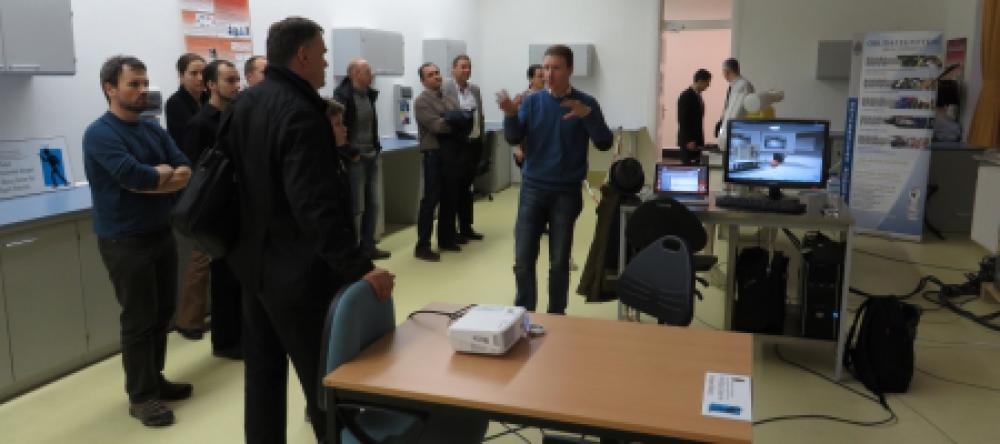
\includegraphics[width=\linewidth]{img/example_fig_1}
		\caption{Example for simple figure}
		\label{fig:example_fig_1}
		\end{figure}

	\end{frame}
	
	\begin{frame}{Example for wrapfigure without caption}
		
		\begin{wrapfigure}{r}{0.3\textwidth} % Its use is a littlebit problematic but not impossible...
			\vspace{-20pt}
			\begin{center}
				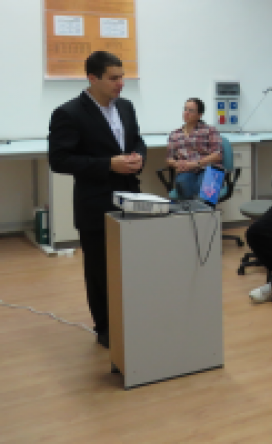
\includegraphics[width=0.3\textwidth]{img/example_fig_2}
				%\caption{Example for \\ wrapfigure}
				\label{fig:example_fig_2}
			\end{center}
			\vspace{-20pt}
			\vspace{1pt}
		\end{wrapfigure} 
		The ABC Center for Intelligent Robotics is devoted to promote the scientific and technological advancement of robotics, primarily for service applications.
		
		\vspace*{2mm}
		
		The ABC Center for Intelligent Robotics was created as a primary reply to the rising demand of integrated education and application-oriented development in robotics. It is an independent platform within the Óbuda University, extensively relying on a national and international network of key partner institutions and companies in Europe and North America, predominantly.

	\end{frame}
	
	\begin{frame}{Example for subfigures}
		\begin{figure}[ht]
			\centering
			\subfigure[Subfigure 1 caption]{
				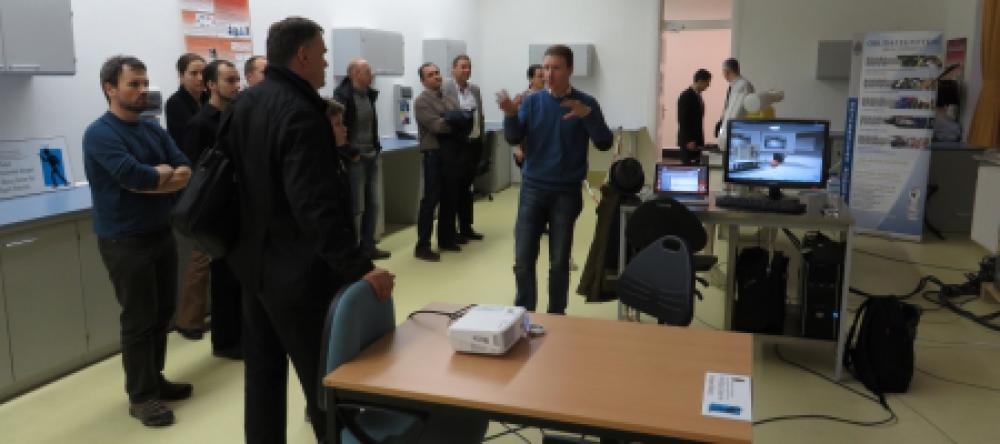
\includegraphics[width = 0.5\textwidth] {img/example_fig_1}
				\label{fig:subfig1}
			} \\
			\subfigure[Subfigure 2 caption]{
				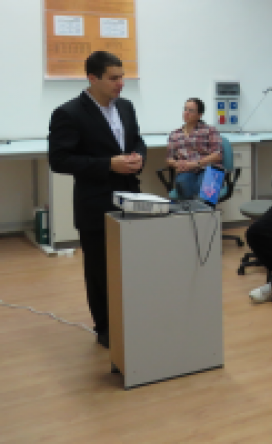
\includegraphics[scale =0.3] {img/example_fig_2}
				\label{fig:subfig2}
			} \hspace{2cm}
			\subfigure[Subfigure 3 caption]{
				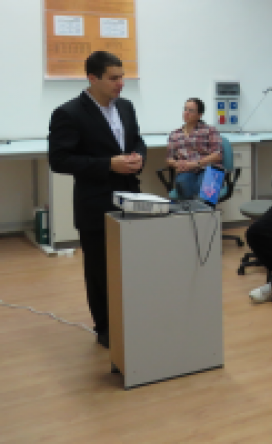
\includegraphics[width = 0.15\textwidth] {img/example_fig_2}
				\label{fig:subfig3}
			}
			\label{myfigure}
			\caption{Global figure caption}
		\end{figure}
	\end{frame}
	
	\begin{frame}
		\frametitle{Examples for}
		\framesubtitle{Mathematical formulas}
		
		A "\texttt{multline}":
		\begin{multline}
		1 + 1+ \\ 1+ 1 + 1 = 5
		\end{multline}
		
		An "\texttt{align*}":
		\begin{align*}
		 1 &= 1 \\
		 1+1&=2 \\
		 1+1+1 &= 3
		\end{align*}
		
		An "\texttt{equation*}" in a "\texttt{block}"
		\begin{block}{Product}
			It is easy to see that
			\begin{equation*}
				\sum_{n=1}^N 1 = N
			\end{equation*}
		\end{block}
		
	\end{frame}
	
	\begin{frame}{Vertical spaces}
		Previous environments are defined with much space before/below them. It can be avoided by using inline equations via \$ \$,
		
		\vspace{3mm}
		
		or commands like \texttt{\textbackslash vspace\{-2mm\}}.
		
		\vspace{3mm}
		
		(With positive arguments the space can be increased.)
	\end{frame}
	
	\begin{frame}{Creating a handout}
		By applying "handout" optional argument as
		"$\backslash$documentclass[handout]{beamer}":
		
		the "$\backslash$pause" comments will not be taken into account
		
		\vspace{5mm}
		
		You can also create a printable form, where three frames are placed into one A4 page by using the command "$\backslash$threeframeslayout"
		
		
		
		\begin{wrapfigure}{r}{0.31\textwidth} % Its use is a littlebit problematic but not impossible...
				\vspace{-8.1mm}
				\fbox{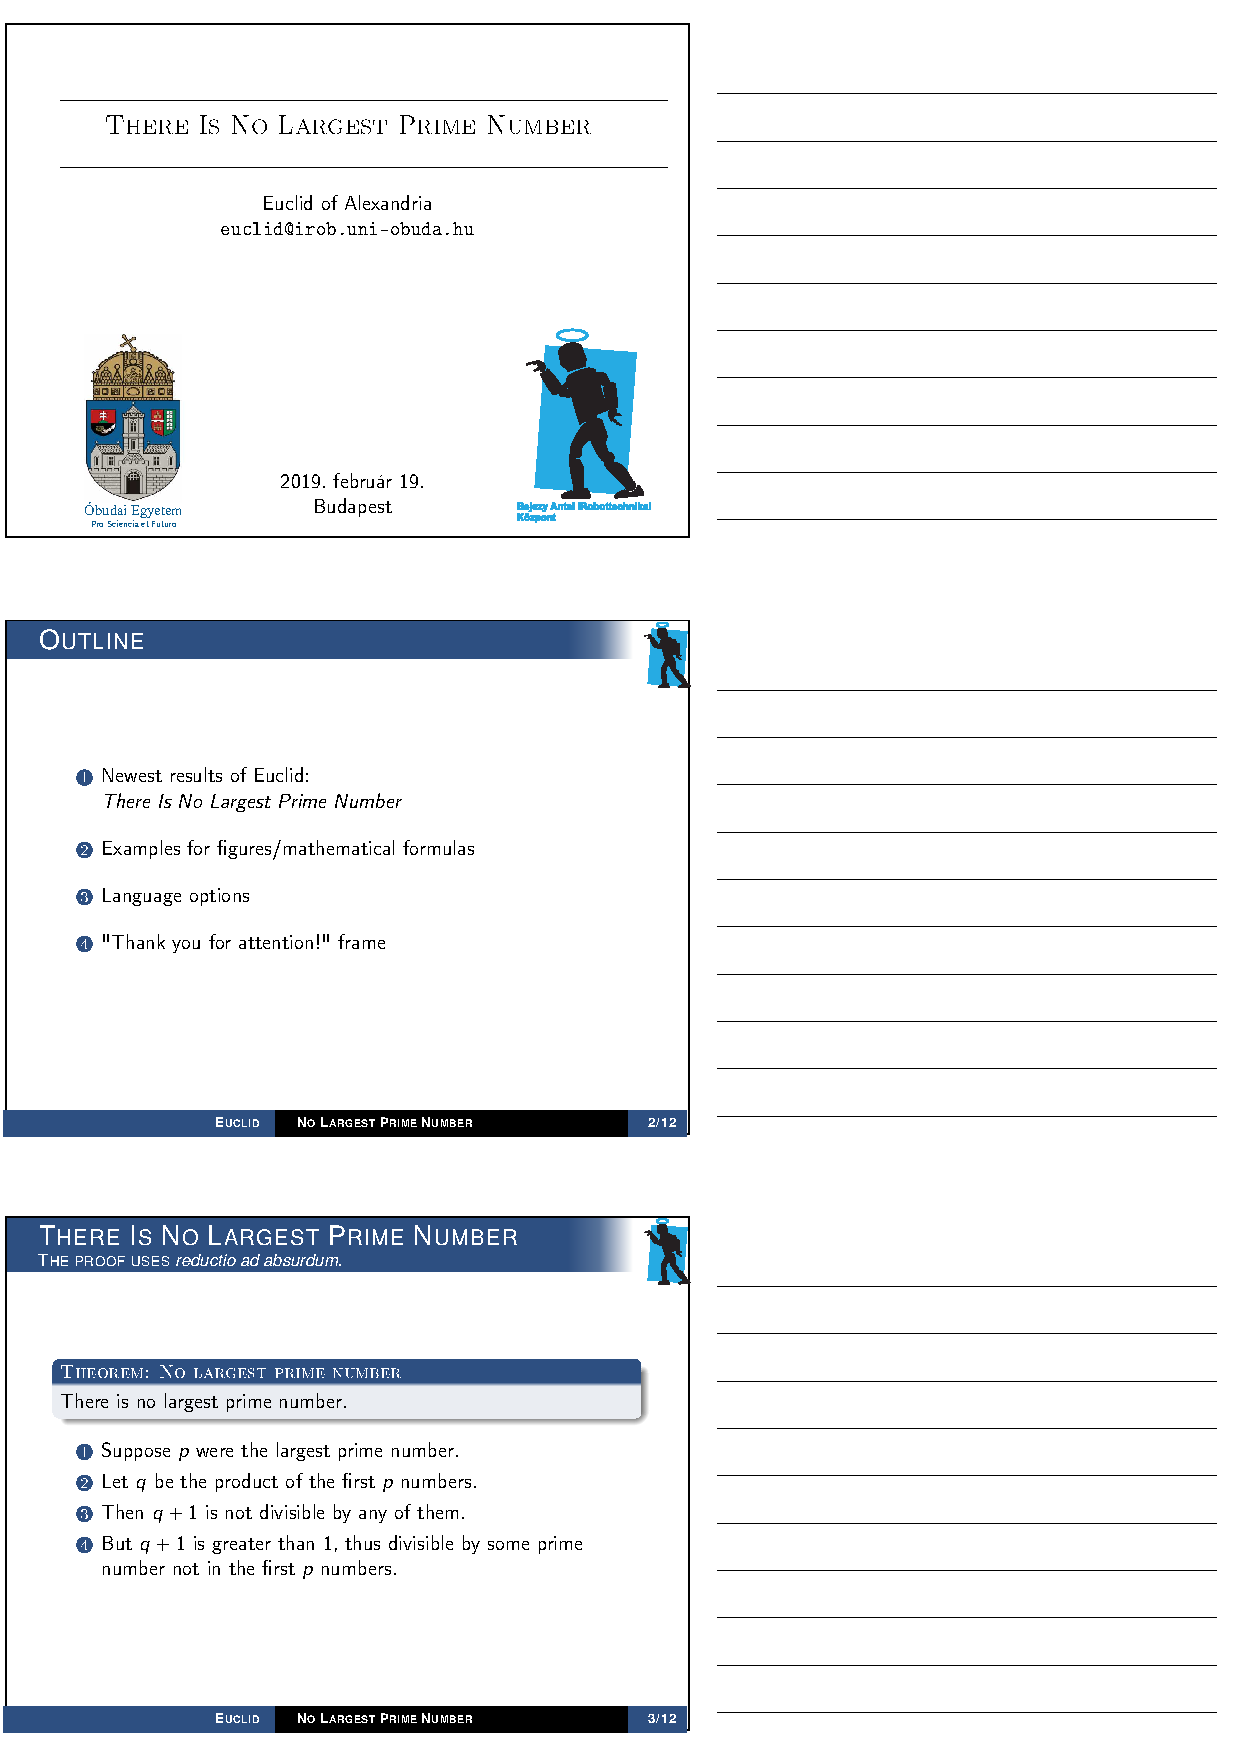
\includegraphics[width=0.3\textwidth]{img/threeframeslayout_example}}
				\vspace{9.1mm}
		\end{wrapfigure} 
	
		\vspace{2mm}
		(In this case, the\\ "thankyouforattentionframe" is omitted \\ to save paper.)
	
		\vspace{5mm}
		
		It is recommended to use it with  the \\ $ $ [handout] option, the result is depicted \\ on the right side
	\end{frame}
	
	\begin{frame}{Example for animation}
	
		The animate package provides opportunity to embed animation into the pdf presentation as
		\animategraphics[controls,width=0.6\textwidth]{5}{img/UR5animation/UR5_pinv--}{1}{36}
		
		For more details, see its documentation: \href{http://mirrors.nxthost.com/ctan/macros/latex/contrib/animate/animate.pdf}{\small http://mirrors.nxthost.com/ctan/macros/latex/contrib/animate/animate.pdf}.
	\end{frame}

	\begin{frame}{Animation compatible with the threeframeslayout}
		A modified animate package is included, that support the threeframeslayout option, if you declare where the animation must be placed: 'top','center' or 'bottom'
		
		The previous animation does not appear in the annotable output, but the next one will be placed appropriately:
		\animategraphics[controls,center,width=0.4\textwidth]{5}{img/UR5animation/UR5_pinv--}{1}{36}
	\end{frame}
	
	\begin{frame}	\showfootline
    \showlogo
    
    
		
		The BARK logo and the footline appear automatically only if there is frametitle defined.
		
		\vspace{3mm}
		
		If it is not defined the \texttt{\textbackslash showfootline} and \texttt{\textbackslash showlogo} commands can be used to show them -- if they are needed -- as in this frame.
		
		\vspace{3mm}
		
		The footline shows the so called shorttitle and shortauthor if they are given (as \texttt{\textbackslash title[A shorttitle]\{A title\}, \textbackslash author[Shortauthors]\{Authors\}}) or the title / author if they are not (as \texttt{\textbackslash title\{A title\}, \textbackslash author\{Authors\}}).
		
	
		
		
	\end{frame}

\begin{frame}

    The font type of titles on the titleframe can be set by applying command:
    \texttt{$\backslash$resettitlefonttype\{cmss\}}
    
    \vspace{10mm}
    
    The font type of title/author/framenumber on normal frames can be set with the command:
    \texttt{$\backslash$resetframetitlefonttype\{cmss\}}
    
    
    \vspace{10mm}
    
    For more details about available latex fontfamilies, see \texttt{https://www.sharelatex.com/learn/Font\_typefaces}
    
    (E.g.: \texttt{phv/cmss/lmbh}...)
    
    \showfootline
    
    \showlogo
\end{frame}
	
	\begin{frame}{Language options}
		
		By using \texttt{\textbackslash usepackage[magyar]\{babel\}} the logos, date format and thanks appear in hungarian, 
		
		\vspace{3mm}
		
		by applying other options, as \texttt{\textbackslash usepackage[english]\{babel\}} they are in english.
		
		\vspace{8mm}
		
		Finally the next dia shows the result of the defined \texttt{\textbackslash thankyouforattentionframe\{The research was supported by...\}} command.
		
	\end{frame}

	

	\thankyouforattentionframe{\footnotesize The research was supported by GP's \& my free time. This very very very very long text is only to check the size of this textbox...\\ By the way, the theme is based on the Warsaw beamer theme of Till Tantau.\\ Best regards, J. Kuti  }
	
\end{document}